\documentclass[12pt]{standalone}

\usepackage{tikz}
\usetikzlibrary{arrows}

\begin{document}

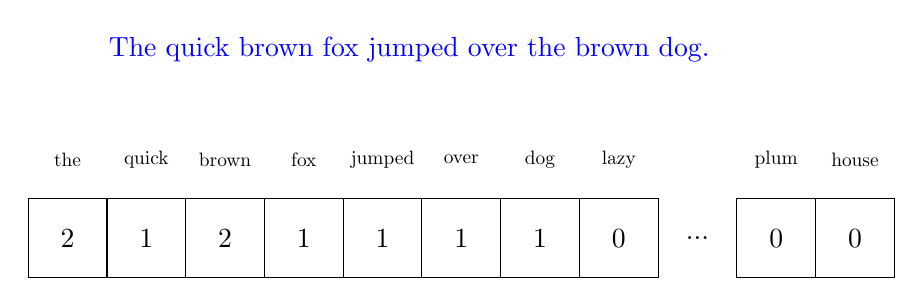
\begin{tikzpicture}

\tikzstyle{count} = [rectangle, minimum size=1cm, draw=black]
\tikzstyle{word} = [scale=0.7]
\tikzstyle{ellipsis} = []

\node[anchor=west,color=blue] at (0.4, 2.4) {The quick brown fox jumped over the brown dog.};

\node[count] at (0, 0) {2};
\node[count] at (1, 0) {1};
\node[count] at (2, 0) {2};
\node[count] at (3, 0) {1};
\node[count] at (4, 0) {1};
\node[count] at (5, 0) {1};
\node[count] at (6, 0) {1};
\node[count] at (7, 0) {0};
\node[ellipsis] at (8, 0) {...};
\node[count] at (9, 0) {0};
\node[count] at (10, 0) {0};

\node[word] at (0, 1) {the};
\node[word] at (1, 1) {quick};
\node[word] at (2, 1) {brown};
\node[word] at (3, 1) {fox};
\node[word] at (4, 1) {jumped};
\node[word] at (5, 1) {over};
\node[word] at (6, 1) {dog};
\node[word] at (7, 1) {lazy};
\node[word] at (9, 1) {plum};
\node[word] at (10, 1) {house};

\end{tikzpicture}

\end{document}
